% ICASSP 2027 manuscript
\documentclass{article}
\usepackage{spconf,amsmath,amssymb,graphicx}
\usepackage[hidelinks]{hyperref}
\usepackage{booktabs}
\emergencystretch=2pt

\title{DSGR-Net: A Differentiable Process-Informed Neural Network for Cotton Yield Response Modeling under Irrigation Management}

\name{Yanyy Yan$^{1,2}$, Liang He$^{1,2,3,4,*}$}
\address{$^{1}$School of Computer Science and Technology, Xinjiang University, Urumqi 830017, China\\
$^{2}$Xinjiang Multimodal Information Technology Engineering Research Center, Urumqi 830017, China\\
$^{3}$School of Intelligence Science and Technology, Xinjiang University, Urumqi 830017, China\\
$^{4}$Department of Electronic Engineering, Tsinghua University, Beijing 100084, China\\
$^{*}$Corresponding author: \texttt{heliang@mail.tsinghua.edu.cn}}

\begin{document}
\ninept
\maketitle

\begin{abstract}
Accurate cotton-yield prediction under irrigation management requires both expressive environmental representations and temporally coherent crop responses. Existing neural predictors learn direct input--yield mappings, whereas crop simulators describe intermediate states but are not optimized jointly with the predictor. To bridge this gap, we propose DSGR-Net, a dual-branch network that couples high-capacity environmental encoding with a differentiable crop-water-growth process. The process branch uses bounded neural corrections to adapt evapotranspiration and radiation-use efficiency, generates daily water-stress and growth trajectories, and encodes them with a stage-aware temporal CNN. A residual gate then integrates process and environmental representations for yield prediction. Experiments on 51,282 DSSAT simulation records show that DSGR-Net achieves $R^2=0.8687\pm0.0280$, RMSE $=450.82\pm41.16$ kg ha$^{-1}$, and MAE $=343.63\pm29.98$ kg ha$^{-1}$. It reduces RMSE by 18.0\% over WL-DNN and by 1.7\% over a strong direct-irrigation DNN, while enabling gradient-based analysis of daily irrigation sensitivity.
\end{abstract}

\begin{keywords}
Cotton yield prediction, differentiable crop model, irrigation response, DSSAT, water stress
\end{keywords}

\section{Introduction}
Cotton production in arid regions is highly dependent on irrigation management. Limited rainfall and strong evaporative demand make yield sensitive not only to the seasonal irrigation amount, but also to when water is supplied~\cite{garibay2019,chen2020,chen2026salinity}. Reliable yield-response modeling must therefore represent the cumulative and stage-dependent effects of daily irrigation rather than reduce a growing season to aggregate management variables.

Process-based crop models provide a mechanistic basis for studying these effects. DSSAT and CSM-CROPGRO-Cotton simulate soil-water balance, phenology, crop stress, biomass, and yield~\cite{jones2003,wang2024}, and support water-efficient and canal-constrained irrigation studies~\cite{garibay2019,wang2025}. Their state trajectories are interpretable, but the simulator normally runs separately from the neural predictor. Its state transitions are therefore not jointly optimized for yield prediction or directly available to gradient-based sensitivity analysis.

Deep learning efficiently maps weather, soil, genotype, and management inputs to yield. Multimodal networks encode simulated environmental and phenological variables~\cite{sajid2025}, while causal-temporal and adjacent-scale attention models capture structured time dependencies~\cite{liu2024ctattn,jiang2024asformer}; related crop studies exploit dynamic states for yield prediction~\cite{moon2023,hao2026}. DSSAT samples also support fast surrogate prediction~\cite{wang2025}. However, these systems commonly connect the crop simulator and neural predictor in an open loop: offline simulated states become fixed features, so yield gradients cannot pass through an explicit irrigation--soil-water--growth pathway.

Physics-guided networks embed biophysical relations into yield estimation~\cite{cao2026}, and AgriPINN introduces differentiable crop-growth constraints under water stress~\cite{agripinn}. Irrigation studies also learn policies from simulated physiological states~\cite{yi2026,chen2025dac,liu2026irl}. Cotton yield response nevertheless requires environmental representation, a differentiable irrigation-to-growth process, and temporal encoding of stage-dependent trajectories to be handled jointly.

We propose DSGR-Net, a differentiable stress-growth response network for cotton yield prediction. A high-capacity branch encodes environmental context, while bounded neural corrections adapt evapotranspiration and radiation-use efficiency within a recurrent crop-water-growth process. A stage-aware temporal CNN encodes the resulting daily trajectories, and residual gated fusion combines them with the environmental representation.

This design differs from static process-feature fusion and a purely neural surrogate. The environmental branch represents broad yield variation across climates and soils, whereas the process branch describes how daily water inputs alter stress and growth. Both branches are optimized by the terminal yield objective, so the learned corrections operate through recurrent crop states rather than independent process labels. The same coupling exposes the contribution of each irrigation event at the output and enables stage-resolved sensitivity analysis without rerunning a separate crop simulator.
Instead of asking the process equations to explain all yield variation, the fusion module lets mechanistic trajectories complement the environmental representation. This separation preserves prediction capacity while making the added process information explicit and testable against direct-irrigation baselines.

The main contributions are summarized as follows:
\begin{itemize}
\item We couple environmental representation learning with a differentiable irrigation--water--stress--growth process.
\item We introduce stage-aware temporal encoding and residual gated fusion for daily process trajectories.
\item We verify the model through grouped yield prediction, cross-year process validation, controlled comparisons, and numerical irrigation-gradient checks.
\end{itemize}

\section{Method}
\label{sec:method}
\subsection{Problem Formulation}
Given a daily sequence of weather and management variables, static soil descriptors, and an irrigation schedule, the objective is to estimate terminal cotton yield while retaining its sensitivity to each daily irrigation input. DSGR-Net models this task with an environmental branch and a recurrent process branch whose representations are jointly decoded into yield.

\subsection{Overall Framework}
Figure~\ref{fig:overview} illustrates the architecture. The environmental branch learns a seasonal representation from weather, soil, and management inputs. In parallel, a recurrent crop-water-growth model generates daily state trajectories with bounded neural corrections. A temporal CNN extracts local and stage-level process patterns, and a residual gate fuses both representations before yield regression.

\begin{figure*}[t]
\centering
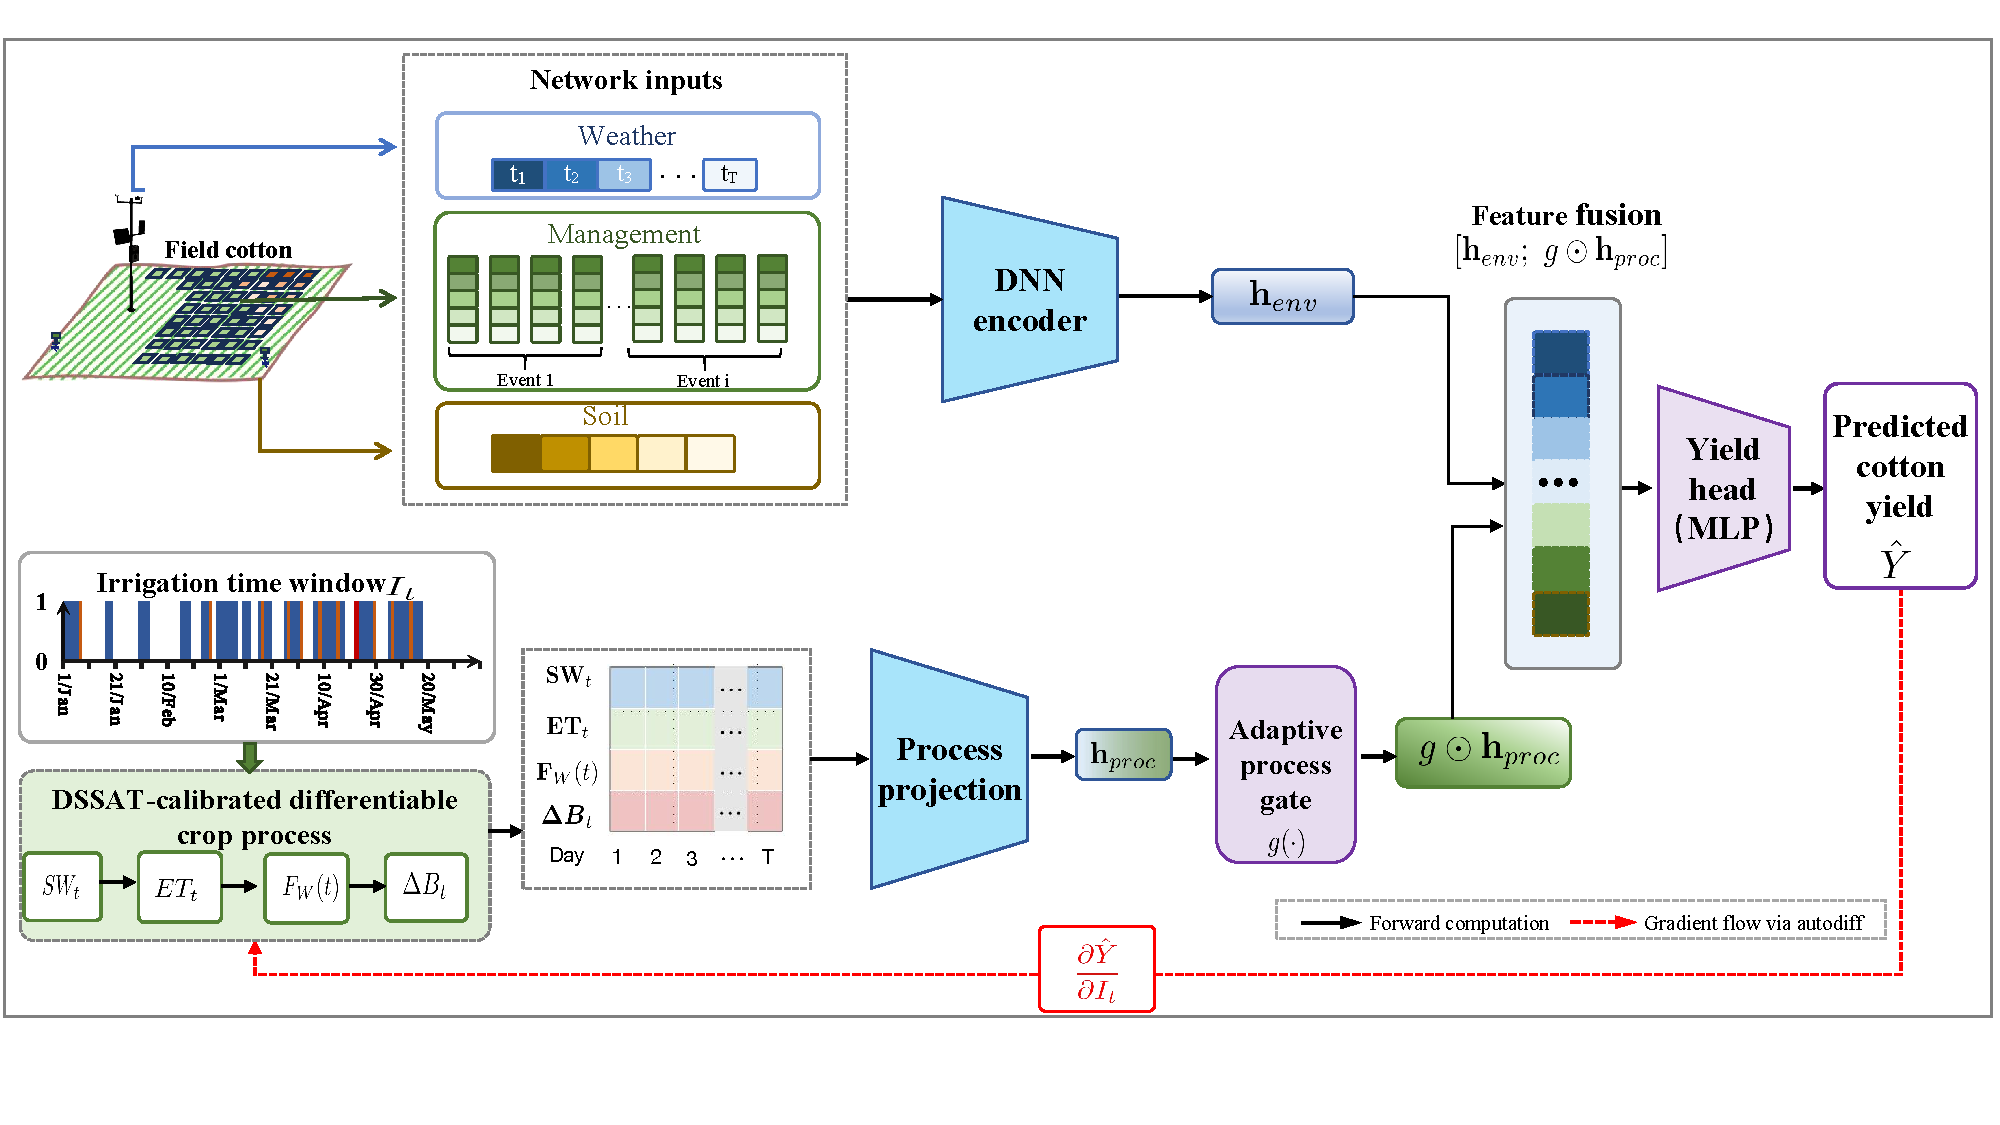
\includegraphics[width=\textwidth]{figures/DSGR_Net_overview.pdf}
\caption{Overview of DSGR-Net. An environmental DNN captures seasonal context, while the process branch generates daily water, stress, and growth states. Stage-aware temporal encoding and residual gated fusion produce the final yield estimate.}
\label{fig:overview}
\end{figure*}

\subsection{Differentiable Water-Stress-Growth Process}
For day $t$, $x_t$ contains nine weather and management variables: solar radiation, maximum and minimum temperature, rainfall, wind, irrigation, and N/P/K application. Static soil and planting descriptors are denoted by $S$. A shared daily DNN produces $h_t$, while a second DNN encodes the masked seasonal sequence and $S$ into the environment embedding $h_{\mathrm{env}}$.

The daily DNN receives $h_t$, the static context, and the recurrent state $(SW_t,B_t,s_t)$, where $s_t$ is normalized thermal development. It estimates bounded relative corrections to evapotranspiration and radiation-use efficiency,
\begin{align}
 \delta_t^{ET}&=0.2\tanh(a_t^{ET}), &
 \delta_t^{RUE}&=0.2\tanh(a_t^{RUE}).
 \label{eq:corrections}
\end{align}
These residuals adapt the calibrated process under changing environment and management while preserving the explicit state recurrence.

The root-zone water state is represented in mm. Let $C$ be the effective storage capacity, $P_t$ rainfall, and $I_t$ irrigation. Water available before daily losses is
\begin{equation}
 SW_t^{+}=SW_t+\eta_P P_t+\eta_I I_t,
 \label{eq:water}
\end{equation}
where $\eta_P=1$ and $\eta_I=0.892$ are calibrated infiltration efficiencies. A radiation-based proxy defines potential evapotranspiration,
\begin{align}
 ET_{0,t}&=0.408\times0.65\,SRAD_t,\\
 ET_t^{d}&=ET_{0,t}K_{c,t}\eta_{ET}(1+\delta_t^{ET})
 \left(0.3+0.7F_{W,t}\right),
\end{align}
where $K_{c,t}=0.3+0.9\sin(\pi s_t)m_t$, $m_t$ is the maturity gate, and $\eta_{ET}=0.959$. Actual ET is limited by available water, and smooth drainage removes a fraction $\rho_D=0.05$ of water above $C$:
\begin{equation}
 ET_t=\min(ET_t^d,SW_t^{+}),\qquad
 SW_{t+1}=SW_t^{+}-ET_t-D_t.
 \label{eq:water_update}
\end{equation}
The growth water-stress factor is computed from the pre-loss water state,
\begin{equation}
 F_{W,t}=\sigma\!\left[k_W(SW_t^{+}/C-\theta_W)\right],
 \qquad 0<F_{W,t}<1,
 \label{eq:fw}
\end{equation}
with calibrated threshold $\theta_W=0.658$ and slope $k_W=2.933$. Water stress is therefore a deterministic function of the recurrent soil-water state rather than a free neural latent variable.

Let $PAR_t$ be the photosynthetically active radiation and $LAI_t$ a bounded phenological canopy function. Absorbed PAR and daily biomass gain are
\begin{align}
 APAR_t &= PAR_t\left(1-\exp(-k_L LAI_t)\right),\\
 \Delta B_t &= RUE_0(1+\delta_t^{RUE})\,APAR_t\,F_{W,t}\,F_{T,t}\,m_t,\\
 B_{t+1} &= B_t+\Delta B_t,
 \label{eq:growth}
\end{align}
where $RUE_0=2.634$ g MJ$^{-1}$, $F_{T,t}$ is a triangular temperature response, and $m_t$ is a smooth gate around 2600 growing-degree days. The recurrence produces an interpretable biomass trajectory; final yield is predicted only after the process trajectory is encoded and fused with the environmental branch.

\subsection{Stage-Aware Process Encoding and Fusion}
The four-channel process sequence is
\begin{equation}
 z_t=\left[SW_t/C,\;ET_t/10,\;F_{W,t},\;\Delta B_t/200\right].
 \label{eq:process_state}
\end{equation}
A 1-D CNN with channel widths $32$--$64$--$64$ extracts local temporal patterns. CNN outputs are averaged within four thermal-development intervals, concatenated, and projected to a 32-dimensional process embedding $h_{\mathrm{proc}}$. A scalar residual gate is defined as
\begin{align}
 q&=\tanh\!\left(G([h_{\mathrm{env}};h_{\mathrm{proc}}])\right),\\
 \tilde h_{\mathrm{proc}}&=(1+0.25q)h_{\mathrm{proc}},\\
 \hat Y&=\mu_Y+\sigma_Y H([h_{\mathrm{env}};\tilde h_{\mathrm{proc}}]),
 \label{eq:yield}
\end{align}
where the gate restricts the process scale to $[0.75,1.25]$. The yield head $H$ is a $64$--$32$ MLP. Irrigation contributes to both the environmental representation and the recurrent process states.

Training minimizes the terminal yield error
\begin{equation}
 \mathcal L_Y=\frac{1}{N}\sum_i(\hat Y_i-Y_i^{\mathrm{obs}})^2.
\end{equation}
Training combines the standardized yield error with a correction regularizer,
\begin{equation}
 \mathcal L=\mathcal L_Y+10^{-3}\mathcal L_{\delta},\qquad
 \mathcal L_{\delta}=\frac{1}{2T_a}\sum_{t\in\mathcal A}
 \left[(\delta_t^{ET})^2+(\delta_t^{RUE})^2\right],
 \label{eq:loss}
\end{equation}
where $\mathcal A$ is the active crop period and $T_a=|\mathcal A|$. The process equations define the recurrent state transitions, while the correction penalty limits departures from the calibrated dynamics. The irrigation sensitivity
\begin{equation}
 \frac{\partial \hat Y}{\partial I_t}
\end{equation}
is obtained from the trained model and characterizes the local change in predicted yield with respect to irrigation applied on day $t$.

\section{Experiment}
In this section, we evaluate DSGR-Net to answer three questions: (1) how accurately does the model predict cotton yield compared with direct neural baselines? (2) does the differentiable process branch provide information beyond direct irrigation features? and (3) can the trained model produce numerically consistent daily irrigation gradients?

\subsection{Experimental Setup}
The clean DSSAT simulation archive contains 51,282 records from 518 environment groups and 99 management scenarios per group. For each random seed, group-wise splitting produces 363/78/77 training/validation/test environments (35,937/7,722/7,623 samples), preventing scenarios from the same environment from crossing splits. All compared models use the same grouped split and training statistics.

Water-process parameters are calibrated with 2022 DSSAT trajectories and frozen for the 2023 check. DSGR-Net is trained with AdamW, batch size 1024, learning rate $5\times10^{-4}$, at most 30 epochs, and early-stopping patience 8. Results are reported over seeds 42, 43, and 44.

We report RMSE, MAE, and $R^2$ for yield and RMSE for the frozen process check. The model comparison separates improvements from stronger environmental encoding, direct irrigation features, process-state encoding, and residual process gating. For each seed, irrigation gradients are checked on eight records, three seasonal dates, and perturbations of 0.01, 0.1, and 1.0 mm. Central differences are used at positive irrigation inputs and forward differences at the zero boundary.

\subsection{Comparative Experiments}
We first examine whether the recurrent water dynamics retain cross-year consistency before assessing terminal yield. Table~\ref{tab:process} reports the 2023 process check using parameters calibrated on 2022 trajectories and then kept fixed. The small SWXD bias indicates that the recurrence preserves the seasonal root-zone water level, while the ETAA result measures the remaining discrepancy in daily atmospheric water loss.

\begin{table}[t]
\centering
\caption{Frozen 2023 process validation after 2022 calibration.}
\label{tab:process}
\begin{tabular}{lcc}
\toprule
Quantity & RMSE & Bias\\
\midrule
SWXD (mm) & 40.069 & $-2.331$ mm\\
ETAA (mm d$^{-1}$) & 1.665 & $-0.414$ mm d$^{-1}$\\
\bottomrule
\end{tabular}
\end{table}

Table~\ref{tab:yield} compares all models using means and sample standard deviations over the same three seeds. WL-DNN is the DNN surrogate adopted from the DSSAT-based irrigation framework of Wang et al.~\cite{wang2025} and serves as the prior-work baseline. DSGR-Net obtains the highest mean $R^2$ and the lowest mean RMSE and MAE. Relative to WL-DNN, it increases $R^2$ by 0.0637 and reduces RMSE and MAE by 18.0\% and 19.6\%, respectively. It also improves over Irrigation-aware DNN by 1.7\% RMSE and 3.5\% MAE, showing that the process trajectory contributes beyond exposing irrigation directly to the neural predictor.

\begin{table}[t]
\centering
\caption{Grouped test-set results, averaged over seeds 42, 43, and 44. Best results are in bold.}
\label{tab:yield}
\scriptsize
\setlength{\tabcolsep}{2.2pt}
\resizebox{\columnwidth}{!}{%
\begin{tabular}{lcc}
\toprule
Model & Test $R^2\!\uparrow$ (RMSE$\!\downarrow$) & MAE$\!\downarrow$\\
\midrule
WL-DNN~\cite{wang2025} & $0.8050\pm0.0384$ ($549.99\pm41.27$) & $427.66\pm47.60$\\
Strong DNN & $0.8444\pm0.0406$ ($489.43\pm57.01$) & $375.13\pm39.95$\\
Irrigation-aware DNN & $0.8631\pm0.0397$ ($458.43\pm59.07$) & $356.09\pm49.73$\\
Process gate (V13) & $0.8632\pm0.0369$ ($458.67\pm54.51$) & $350.74\pm37.75$\\
Gradient-informed NN & $0.8438\pm0.0340$ ($491.60\pm44.37$) & $378.11\pm34.47$\\
Temporal CNN & $0.8454\pm0.0277$ ($489.90\pm34.39$) & $376.47\pm27.74$\\
Multi-scale CNN & $0.8339\pm0.0376$ ($506.63\pm47.17$) & $388.56\pm38.48$\\
Hybrid NN--CNN & $0.8267\pm0.0395$ ($517.54\pm48.14$) & $395.23\pm34.71$\\
\textbf{DSGR-Net (ours)} & $\mathbf{0.8687\pm0.0280}$ ($\mathbf{450.82\pm41.16}$) & $\mathbf{343.63\pm29.98}$\\
\bottomrule
\end{tabular}%
}
\end{table}

\subsection{Ablation Study}
Table~\ref{tab:ablation} follows a component-wise protocol: the environmental encoder is fixed, while direct irrigation input, differentiable process trajectories, and the fusion rule are introduced successively. This separates architectural contributions from changes in data split or training budget.

\begin{table}[t]
\centering
\caption{Controlled ablation of irrigation input, process trajectory, and fusion.}
\label{tab:ablation}
\scriptsize
\setlength{\tabcolsep}{2.0pt}
\resizebox{\columnwidth}{!}{%
\begin{tabular}{lccccl}
\toprule
Variant & Direct irr. & Process traj. & Fusion & $R^2\!\uparrow$ & RMSE$\!\downarrow$\\
\midrule
Strong DNN & -- & -- & -- & 0.8444 & 489.43\\
Irrigation-aware DNN & $\checkmark$ & -- & -- & 0.8631 & 458.43\\
Process gate (V13) & $\checkmark$ & $\checkmark$ & Sigmoid & 0.8632 & 458.67\\
\textbf{DSGR-Net} & $\checkmark$ & $\checkmark$ & Residual & \textbf{0.8687} & \textbf{450.82}\\
\bottomrule
\end{tabular}%
}
\end{table}

Adding direct irrigation reduces RMSE from 489.43 to 458.43 kg ha$^{-1}$ and raises $R^2$ from 0.8444 to 0.8631. Replacing direct-input-only prediction with a sigmoid-gated process trajectory gives similar RMSE, while reducing MAE from 356.09 to 350.74 kg ha$^{-1}$. The final residual fusion further reduces RMSE to 450.82 kg ha$^{-1}$ and MAE to 343.63 kg ha$^{-1}$. Thus, the gain comes from the combination of explicit process-state encoding and bounded residual fusion rather than from irrigation input alone.

Across the three seeds, all 216 audited irrigation gradients are finite. The median relative error between automatic differentiation and numerical differences is $3.26\times10^{-5}$, $9.28\times10^{-5}$, and $1.19\times10^{-4}$ for seeds 42--44, respectively. These results confirm that daily irrigation sensitivity can be evaluated consistently in the proposed model.

Figure~\ref{fig:irrigation_gradient} summarizes the resulting irrigation response. Sensitivity concentrates in the middle of the season and reaches its maximum near DAP 89. At the growth-stage level, flowering has the largest mean response, followed by boll filling, whereas sensitivity is low during maturity. This pattern shows that DSGR-Net learns a nonlinear and stage-dependent irrigation response rather than assigning a uniform contribution to seasonal irrigation.

\begin{figure}[t]
\centering
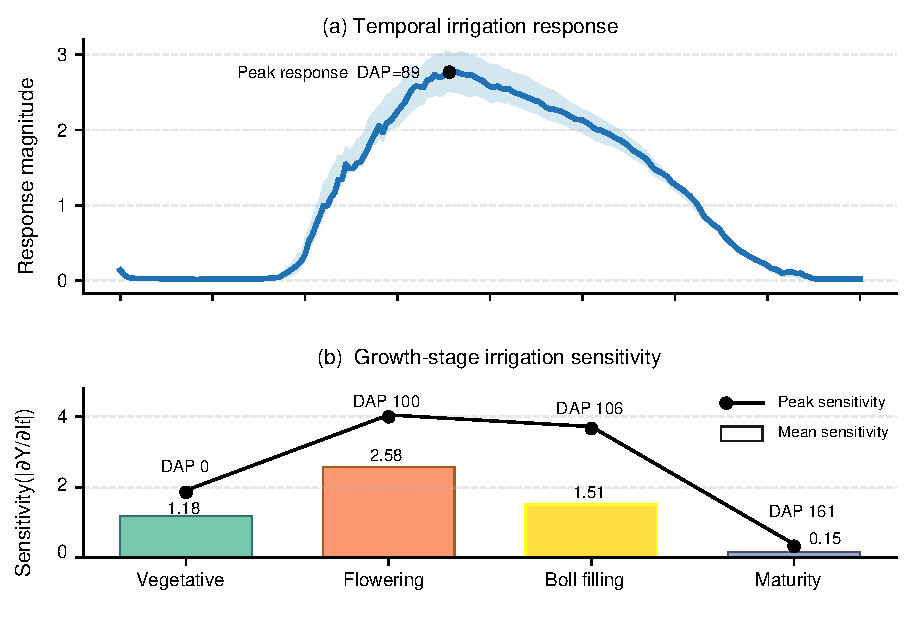
\includegraphics[width=\columnwidth]{figures/irrigation_gradient_analysis.pdf}
\caption{Temporal irrigation response and growth-stage sensitivity. The shaded band in (a) summarizes variation in the daily response, and (b) reports mean and peak sensitivity within each stage.}
\label{fig:irrigation_gradient}
\end{figure}

\section{Conclusion}
We presented DSGR-Net, a differentiable crop-process-guided network for cotton yield response under irrigation management. It combines environmental representation learning, recurrent water--stress--growth modeling, temporal process encoding, and residual gated fusion. DSGR-Net achieves $R^2=0.8687$, RMSE $=450.82$ kg ha$^{-1}$, and MAE $=343.63$ kg ha$^{-1}$ on the grouped test set, outperforming the direct-irrigation DNN while supporting daily irrigation-sensitivity analysis.

\begin{thebibliography}{00}
\bibitem{garibay2019}
V. M. Garibay, K. Kothari, S. Ale, D. C. Gitz, G. D. Morgan, and C. L. Munster, ``Determining water-use-efficient irrigation strategies for cotton using the DSSAT CSM CROPGRO-Cotton model evaluated with in-season data,'' \emph{Agric. Water Manag.}, vol. 223, Art. no. 105695, Aug. 2019, doi: 10.1016/j.agwat.2019.105695.

\bibitem{chen2020}
X. Chen et al., ``Evaluation of a new irrigation decision support system in improving cotton yield and water productivity in an arid climate,'' \emph{Agric. Water Manag.}, vol. 234, Art. no. 106139, May 2020, doi: 10.1016/j.agwat.2020.106139.

\bibitem{chen2026salinity}
Q. Chen et al., ``Predicting cotton yield and optimizing irrigation scheduling from coupled soil water--salinity dynamics,'' \emph{Agric. Water Manag.}, vol. 334, Art. no. 110695, Sep. 2026, doi: 10.1016/j.agwat.2026.110695.

\bibitem{jones2003}
J. W. Jones et al., ``The DSSAT cropping system model,'' \emph{Eur. J. Agron.}, vol. 18, nos. 3--4, pp. 235--265, Jan. 2003, doi: 10.1016/S1161-0301(02)00107-7.

\bibitem{wang2024}
L. Wang, M. Lin, Z. Han, L. Han, L. He, and W. Sun, ``Simulating the effects of drought stress timing and the amount irrigation on cotton yield using the CSM-CROPGRO-Cotton model,'' \emph{Agronomy}, vol. 14, no. 1, Art. no. 14, Jan. 2024, doi: 10.3390/agronomy14010014.

\bibitem{wang2025}
L. Wang, L. He, W. Sun, C. Gao, Z. Han, and M. Lin, ``Precise irrigation of dryland cotton under canal irrigation system constraints based on the CERES-CROPGRO-Cotton model,'' \emph{Agric. Water Manag.}, vol. 317, Art. no. 109624, Aug. 2025, doi: 10.1016/j.agwat.2025.109624.

\bibitem{sajid2025}
S. S. Sajid, Z. Khalilzadeh, L. Wang, and G. Hu, ``Analyses of crop yield dynamics and the development of a multimodal neural network prediction model with G$\times$E$\times$M interactions,'' \emph{Front. Plant Sci.}, vol. 16, Jul. 2025, doi: 10.3389/fpls.2025.1537990.

\bibitem{liu2024ctattn}
W. Liu, Y. He, J. Guan, and S. Zhou, ``Multivariate time series forecasting with causal-temporal attention network,'' in \emph{Proc. IEEE Int. Conf. Acoust., Speech Signal Process. (ICASSP)}, Seoul, Republic of Korea, 2024, pp. 5735--5739, doi: 10.1109/ICASSP48485.2024.10448031.

\bibitem{jiang2024asformer}
H. Jiang, Z. Chen, W. Ding, and F. Lin, ``ASformer: Learning from adjacent scale,'' in \emph{Proc. IEEE Int. Conf. Acoust., Speech Signal Process. (ICASSP)}, Seoul, Republic of Korea, 2024, pp. 5900--5904, doi: 10.1109/ICASSP48485.2024.10445968.

\bibitem{moon2023}
T. Moon, D. Kim, S. Kwon, and J. E. Son, ``Process-based crop modeling for high applicability with attention mechanism and multitask decoders,'' \emph{Plant Phenomics}, vol. 5, Art. no. 0035, 2023, doi: 10.34133/plantphenomics.0035.

\bibitem{hao2026}
D. Hao, L. Chen, G. Chen, C. Chen, Q. Zhu, and L. Zhangzhong, ``Improving maize yield prediction performance via a hybrid framework coupling an optimized crop model and deep learning,'' \emph{Agric. Syst.}, vol. 236, Art. no. 104768, Jun. 2026, doi: 10.1016/j.agsy.2026.104768.

\bibitem{cao2026}
B. Cao et al., ``Physics-guided deep learning for crop yield estimation,'' \emph{Eur. J. Agron.}, vol. 172, Art. no. 127850, Jan. 2026, doi: 10.1016/j.eja.2025.127850.

\bibitem{agripinn}
Y. Shi et al., ``AgriPINN: A process-informed neural network for interpretable and scalable crop biomass prediction under water stress,'' arXiv:2601.16045, 2026, doi: 10.48550/arXiv.2601.16045.

\bibitem{yi2026}
Z. Yi, Z. Fang, R. Xu, S. Yuan, and L. He, ``PROSE: Probabilistic reinforcement learning optimized by success estimation for stage-aware cotton irrigation scheduling,'' in \emph{Proc. IEEE Int. Conf. Acoust., Speech Signal Process. (ICASSP)}, 2026, doi: 10.1109/ICASSP55912.2026.11461289.

\bibitem{chen2025dac}
Y. Chen, M. Lin, Z. Yu, W. Sun, W. Fu, and L. He, ``Enhancing cotton irrigation with distributional actor--critic reinforcement learning,'' \emph{Agric. Water Manag.}, vol. 307, Art. no. 109194, Feb. 2025, doi: 10.1016/j.agwat.2024.109194.

\bibitem{liu2026irl}
K. Liu, A. Xu, and G. Liu, ``An interpretable agent integrating offline imitation and reinforcement learning for cotton irrigation scheduling,'' \emph{Eur. J. Agron.}, vol. 179, Art. no. 128153, Aug. 2026, doi: 10.1016/j.eja.2026.128153.

\end{thebibliography}

\end{document}
